\documentclass[aspectratio=169,11pt]{beamer}

% ============================================================
% SISMID 2026 -- Day 1, 1:30 session
% Google Trends in depth (S. Yang + C. Djorno)
% Part A: nuts, bolts, gotchas + statistical preprocessing
%   (Djorno et al., Restoring the Forecasting Power of Google
%    Trends with Statistical Preprocessing, IJF 2026)
% Part B: retrieving related queries to complete the picture
%   (Djorno, Slavin, Yang, Meyer, Santillana, in progress:
%    search behavior reveals a three-stage temporal structure)
% Compile: pdflatex google-trends-in-depth.tex  (run twice)
% ============================================================

\IfFileExists{beamerthememetropolis.sty}{
  \usetheme{metropolis}
  \metroset{progressbar=frametitle, sectionpage=progressbar, numbering=fraction}
}{
  \usetheme{Boadilla}
  \usecolortheme{seahorse}
  \setbeamertemplate{navigation symbols}{}
}

\usepackage[utf8]{inputenc}
\usepackage[T1]{fontenc}
\usepackage{tikz}
\usetikzlibrary{arrows.meta, positioning, fit, backgrounds, calc}
\usepackage{xcolor}
\usepackage{graphicx}
\usepackage{amsmath}
\usepackage{booktabs}

\definecolor{AccentA}{HTML}{2A6F97}
\definecolor{AccentB}{HTML}{C1666B}
\definecolor{AccentC}{HTML}{3B8A5B}
\setbeamercolor{frametitle}{bg=AccentA}
\setbeamercolor{progress bar}{fg=AccentB}

\tikzset{
  cbox/.style={draw=AccentA, very thick, rounded corners, align=center,
    minimum height=1.0cm, inner sep=6pt, font=\small, fill=AccentA!6},
  sbox/.style={draw=AccentA, thick, rounded corners, align=center,
    minimum height=0.85cm, inner sep=4pt, font=\scriptsize, fill=AccentA!6},
  rbox/.style={draw=AccentB, thick, rounded corners, align=center,
    minimum height=0.85cm, inner sep=4pt, font=\scriptsize, fill=AccentB!8},
  gbox/.style={draw=AccentC, thick, rounded corners, align=center,
    minimum height=0.85cm, inner sep=4pt, font=\scriptsize, fill=AccentC!8},
  flow/.style={-{Stealth[length=3mm]}, very thick, draw=AccentB},
  flowq/.style={-{Stealth[length=2.4mm]}, thick, draw=AccentA!70},
}

\title{Google Trends in Depth}
\subtitle{The nuts, the bolts, and the gotchas}
\author{Shihao Yang \quad\textbullet\quad Candice Djorno}
\institute{SISMID 2026 \textbullet\ Day 1, 1:30}
\date{July 20, 2026}

\begin{document}

\begin{frame}
  \titlepage
\end{frame}

\begin{frame}{Why a whole session on one data source}
  You scraped it this morning and modeled with it before lunch. Now the fine print.
  \begin{itemize}
    \item Google Trends is the backbone signal of digital epidemiology, and it is
          \textbf{deceptively messy}. Used naively, it can \emph{hurt} a forecast.
    \item Two halves, both from our own work:
      \begin{itemize}
        \item \textbf{The gotchas and the fix}: how the data is really generated, and how
              to preprocess it so it forecasts again.
        \item \textbf{Completing the picture}: how to find the \emph{right} related
              queries, and what they reveal about disease progression.
      \end{itemize}
  \end{itemize}
  \vspace{0.3em}
  \begin{center}
    \itshape The goal: leave able to spot a bad Google Trends signal, and to fix it.
  \end{center}
\end{frame}

\begin{frame}{Roadmap}
  \tableofcontents
\end{frame}

% ===============================================================
\section{What Google Trends actually is}

\begin{frame}{It is not a search count}
  Google Trends never gives you the number of searches. It gives \textbf{relative
  interest}, and that changes everything.
  \begin{itemize}
    \item Values are scaled \textbf{0 to 100} \emph{within} the query set, time window,
          and geography you asked for. Change any of those and every number moves.
    \item It is computed from a \textbf{random sample} of Google searches, re-drawn each
          time. Pull the same query twice and you can get different numbers.
    \item Low volumes are rounded, and below a privacy threshold they are reported as
          \textbf{zero}.
  \end{itemize}
  \vspace{0.3em}
  \begin{center}
    \itshape A single raw pull is one noisy, rescaled, partly censored draw. Not the truth.
  \end{center}
\end{frame}

\begin{frame}{How a Google Trends value is made}
  \begin{center}
  \resizebox{0.98\textwidth}{!}{%
  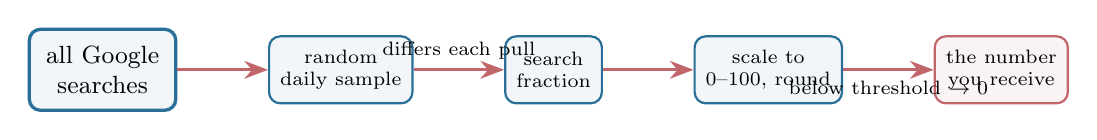
\begin{tikzpicture}[node distance=1.15cm]
    \node[cbox] (all) {all Google\\searches};
    \node[sbox, right=of all] (samp) {random\\daily sample};
    \node[sbox, right=of samp] (frac) {search\\fraction};
    \node[sbox, right=of frac] (scale) {scale to\\0--100, round};
    \node[rbox, right=of scale] (you) {the number\\you receive};
    \draw[flow] (all) -- (samp);
    \draw[flow] (samp) -- node[above,font=\scriptsize]{differs each pull} (frac);
    \draw[flow] (frac) -- (scale);
    \draw[flow] (scale) -- node[below,font=\scriptsize]{below threshold $\to 0$} (you);
  \end{tikzpicture}}
  \end{center}
  \vspace{0.5em}
  \begin{itemize}
    \item Every step that makes it privacy-safe and comparable also makes it
          \textbf{unstable}: sampling, rounding, thresholding, rescaling.
    \item So cleaning it up is a \textbf{statistics problem}, not an engineering one.
  \end{itemize}
\end{frame}

% ===============================================================
\section{The four gotchas}

\begin{frame}{Raw Google Trends has four structural problems}
  From \emph{Restoring the Forecasting Power of Google Trends with Statistical
  Preprocessing} (Djorno, Yang, et al., \emph{IJF} 2026):
  \begin{enumerate}
    \item \textbf{Missing values} (zeros from the privacy threshold),
    \item \textbf{Sampling variability} (different numbers across downloads),
    \item \textbf{Noise} (jitter even in non-zero series),
    \item \textbf{Trend} (magnitudes shift when Google changes its pipeline).
  \end{enumerate}
  \vspace{0.4em}
  \begin{alertblock}{And it is getting worse}
    Quality has \textbf{deteriorated} recently: more zeros and more noise, even for
    queries that used to be stable. Old code that worked in 2016 can quietly fail now.
  \end{alertblock}
\end{frame}

\begin{frame}{Gotcha 1: zeros from the privacy threshold}
  \begin{columns}[T]
    \begin{column}{0.58\textwidth}
      \begin{itemize}
        \item Search volumes below a privacy cutoff are reported as \textbf{0}, not as a
              small number.
        \item A modestly popular term (say ``influenza treatment'') can come back
              \textbf{mostly zeros}, especially at the state level or off-season.
        \item Those zeros are not ``no interest''; they are \textbf{censored} data. Feed
              them to a model as real values and you teach it nonsense.
      \end{itemize}
    \end{column}
    \begin{column}{0.4\textwidth}
      \begin{block}{Tell-tale sign}
        A column that is $>50$--$80\%$ zeros. Standard move: drop columns with
        $>80\%$ zeros, or combine terms to lift them above the threshold (later).
      \end{block}
    \end{column}
  \end{columns}
\end{frame}

\begin{frame}{Gotcha 2: sampling variability}
  \begin{itemize}
    \item The 0--100 series is built from a \textbf{fresh random sample} each time Google
          computes it. Two downloads of the same query, on different days, \textbf{disagree}.
    \item This is not rounding. The underlying draw is different, so historical values you
          pulled last month may not match what you pull today.
  \end{itemize}
  \vspace{0.4em}
  \begin{block}{Consequence for you}
    Your ``data'' is a random variable. A model fit on one pull is fit on one realization.
    The cure is to treat it like sampling: \textbf{pull repeatedly and average}, so the
    noise cancels.
  \end{block}
\end{frame}

\begin{frame}{Gotchas 3 and 4: noise and trend}
  \begin{columns}[T]
    \begin{column}{0.5\textwidth}
      \textbf{Noise}
      \begin{itemize}
        \item Even a clean, non-zero series jitters week to week beyond real behavior.
        \item Low signal-to-noise swamps the actual epidemic signal.
      \end{itemize}
    \end{column}
    \begin{column}{0.5\textwidth}
      \textbf{Trend (the sneaky one)}
      \begin{itemize}
        \item Google periodically changes its data collection (it even annotates this on
              the site).
        \item Magnitudes drift over the years for reasons that have \emph{nothing} to do
              with searching. A spurious trend the model will happily fit.
      \end{itemize}
    \end{column}
  \end{columns}
  \vfill
  \begin{center}
    \itshape Four different problems. They need four different, deliberate fixes.
  \end{center}
\end{frame}

% ===============================================================
\section{The fix: statistical preprocessing}

\begin{frame}{Three fixes, and a headline result}
  The Restoring recipe: \textbf{hierarchical clustering, smoothing splines, detrending}.
  \begin{center}
  \resizebox{0.72\textwidth}{!}{%
  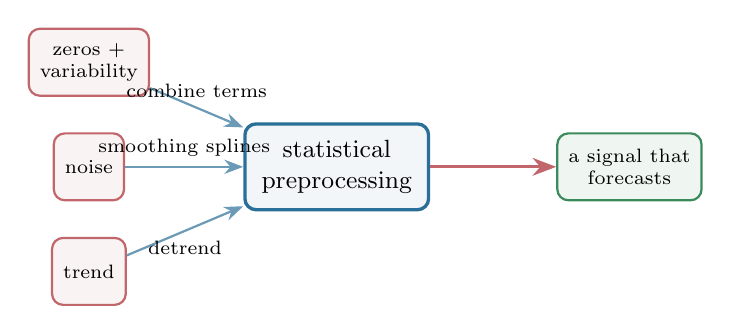
\begin{tikzpicture}[node distance=0.45cm and 1.1cm]
    \node[rbox] (z) {zeros +\\variability};
    \node[rbox, below=of z] (n) {noise};
    \node[rbox, below=of n] (t) {trend};
    \node[cbox, right=1.5cm of n, yshift=0cm] (fix) {statistical\\preprocessing};
    \node[gbox, right=1.6cm of fix] (out) {a signal that\\forecasts};
    \draw[flowq] (z) -- node[above,font=\scriptsize]{combine terms} (fix);
    \draw[flowq] (n) -- node[above,font=\scriptsize]{smoothing splines} (fix);
    \draw[flowq] (t) -- node[below,font=\scriptsize]{detrend} (fix);
    \draw[flow] (fix) -- (out);
  \end{tikzpicture}}
  \end{center}
  \vspace{0.2em}
  \begin{center}
    \itshape Validated by forecasting U.S. flu hospitalizations with ARIMAX: raw Google
    Trends \textbf{hurt}; preprocessed improved accuracy \textbf{58\% nationally, 24\% by
    state}.
  \end{center}
\end{frame}

\begin{frame}{Fix 1: combine related terms (beats zeros and variability)}
  \begin{itemize}
    \item Cluster related queries, then \textbf{sum} them into one series (Google's Boolean
          additive query, \texttt{term1 + term2 + ...}).
    \item Combining lifts low-volume terms \textbf{above the zero threshold}, so the
          censoring problem largely disappears.
    \item Summing many partly-independent draws also \textbf{averages out} the sampling
          noise. One good composite beats many sparse columns.
  \end{itemize}
  \vspace{0.3em}
  \begin{center}
    \itshape This is also the bridge to Part B: which terms belong together?
  \end{center}
\end{frame}

\begin{frame}{Fix 2 and Fix 3: denoise, then detrend}
  \begin{columns}[T]
    \begin{column}{0.5\textwidth}
      \textbf{Denoise (smoothing splines)}
      \begin{itemize}
        \item Fit a smooth curve through the jitter; keep the epidemic-scale signal.
        \item Combined with repeated pulls and averaging, this lifts the
              signal-to-noise ratio substantially.
      \end{itemize}
    \end{column}
    \begin{column}{0.5\textwidth}
      \textbf{Detrend}
      \begin{itemize}
        \item Estimate the slow deterministic drift from pipeline changes and
              \textbf{remove it}.
        \item What remains moves with the disease, not with Google's algorithm updates.
      \end{itemize}
    \end{column}
  \end{columns}
  \vfill
  \begin{block}{The lesson}
    A fancier forecasting model did not rescue Google Trends. \textbf{Careful preprocessing
    did.} Clean the input before you blame the model.
  \end{block}
\end{frame}

% ===============================================================
\section{Completing the picture: related queries}

\begin{frame}{One term is never the whole story}
  From our in-progress work with C. Djorno (Djorno, Slavin, Yang, Meyer, Santillana):
  \begin{itemize}
    \item ``dengue'' or ``flu'' alone captures a slice of behavior. The full outbreak
          shows up across a \textbf{family} of queries: prevention, symptoms, treatment,
          complications.
    \item To see the whole disease, you have to \textbf{find the related queries} and use
          them together, not guess one keyword.
  \end{itemize}
  \vspace{0.3em}
  \begin{center}
    \itshape Retrieving related queries is what makes the Google Trends picture complete.
  \end{center}
\end{frame}

\begin{frame}{Trick: use topics, not raw strings}
  \begin{itemize}
    \item A raw string (``flu'') misses spellings, synonyms, and other languages.
    \item Google Trends \textbf{topics} aggregate semantically equivalent searches across
          spellings and languages into one entity.
    \item Topics carry \textbf{more volume} and \textbf{fewer zeros}, which directly helps
          with Gotcha 1. Prefer topics whenever they exist.
  \end{itemize}
  \vspace{0.3em}
  \begin{block}{How to build the pool}
    Seed with the obvious terms, harvest \textbf{related and rising} queries, and pull
    topic IDs (e.g., from Wikidata). Then filter: drop columns $>80\%$ zeros, and keep
    terms that actually correlate with the disease at some lag.
  \end{block}
\end{frame}

\begin{frame}{Then group them into stage composites}
  \begin{center}
  \resizebox{0.4\textwidth}{!}{%
  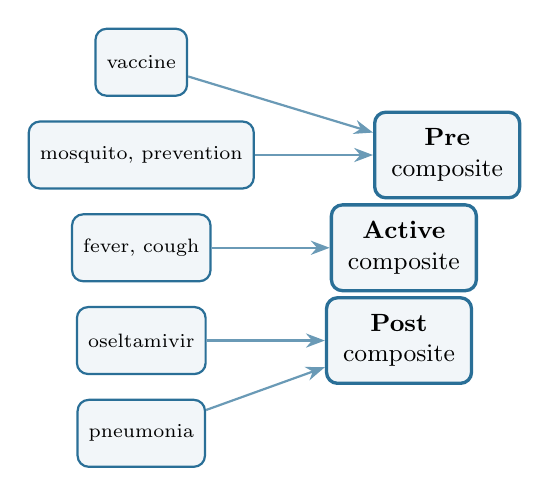
\begin{tikzpicture}[node distance=0.3cm and 1.2cm]
    \node[sbox] (t1) {vaccine};
    \node[sbox, below=of t1] (t2) {mosquito, prevention};
    \node[sbox, below=of t2] (t3) {fever, cough};
    \node[sbox, below=of t3] (t4) {oseltamivir};
    \node[sbox, below=of t4] (t5) {pneumonia};
    \node[cbox, right=1.5cm of t2] (pre) {\textbf{Pre}\\composite};
    \node[cbox, right=1.5cm of t3] (act) {\textbf{Active}\\composite};
    \node[cbox, right=1.5cm of t4] (post) {\textbf{Post}\\composite};
    \draw[flowq] (t1) -- (pre); \draw[flowq] (t2) -- (pre);
    \draw[flowq] (t3) -- (act);
    \draw[flowq] (t4) -- (post); \draw[flowq] (t5) -- (post);
  \end{tikzpicture}}
  \end{center}
  \begin{itemize}
    \item Cluster terms by \textbf{when} they peak relative to cases, then sum each
          cluster into one composite (Fix 1 again).
    \item Result: a few clean, near-orthogonal signals, not hundreds of sparse columns.
  \end{itemize}
\end{frame}

\begin{frame}{The payoff: search encodes a three-stage timeline}
  \begin{columns}[c]
    \begin{column}{0.52\textwidth}
      \centering
      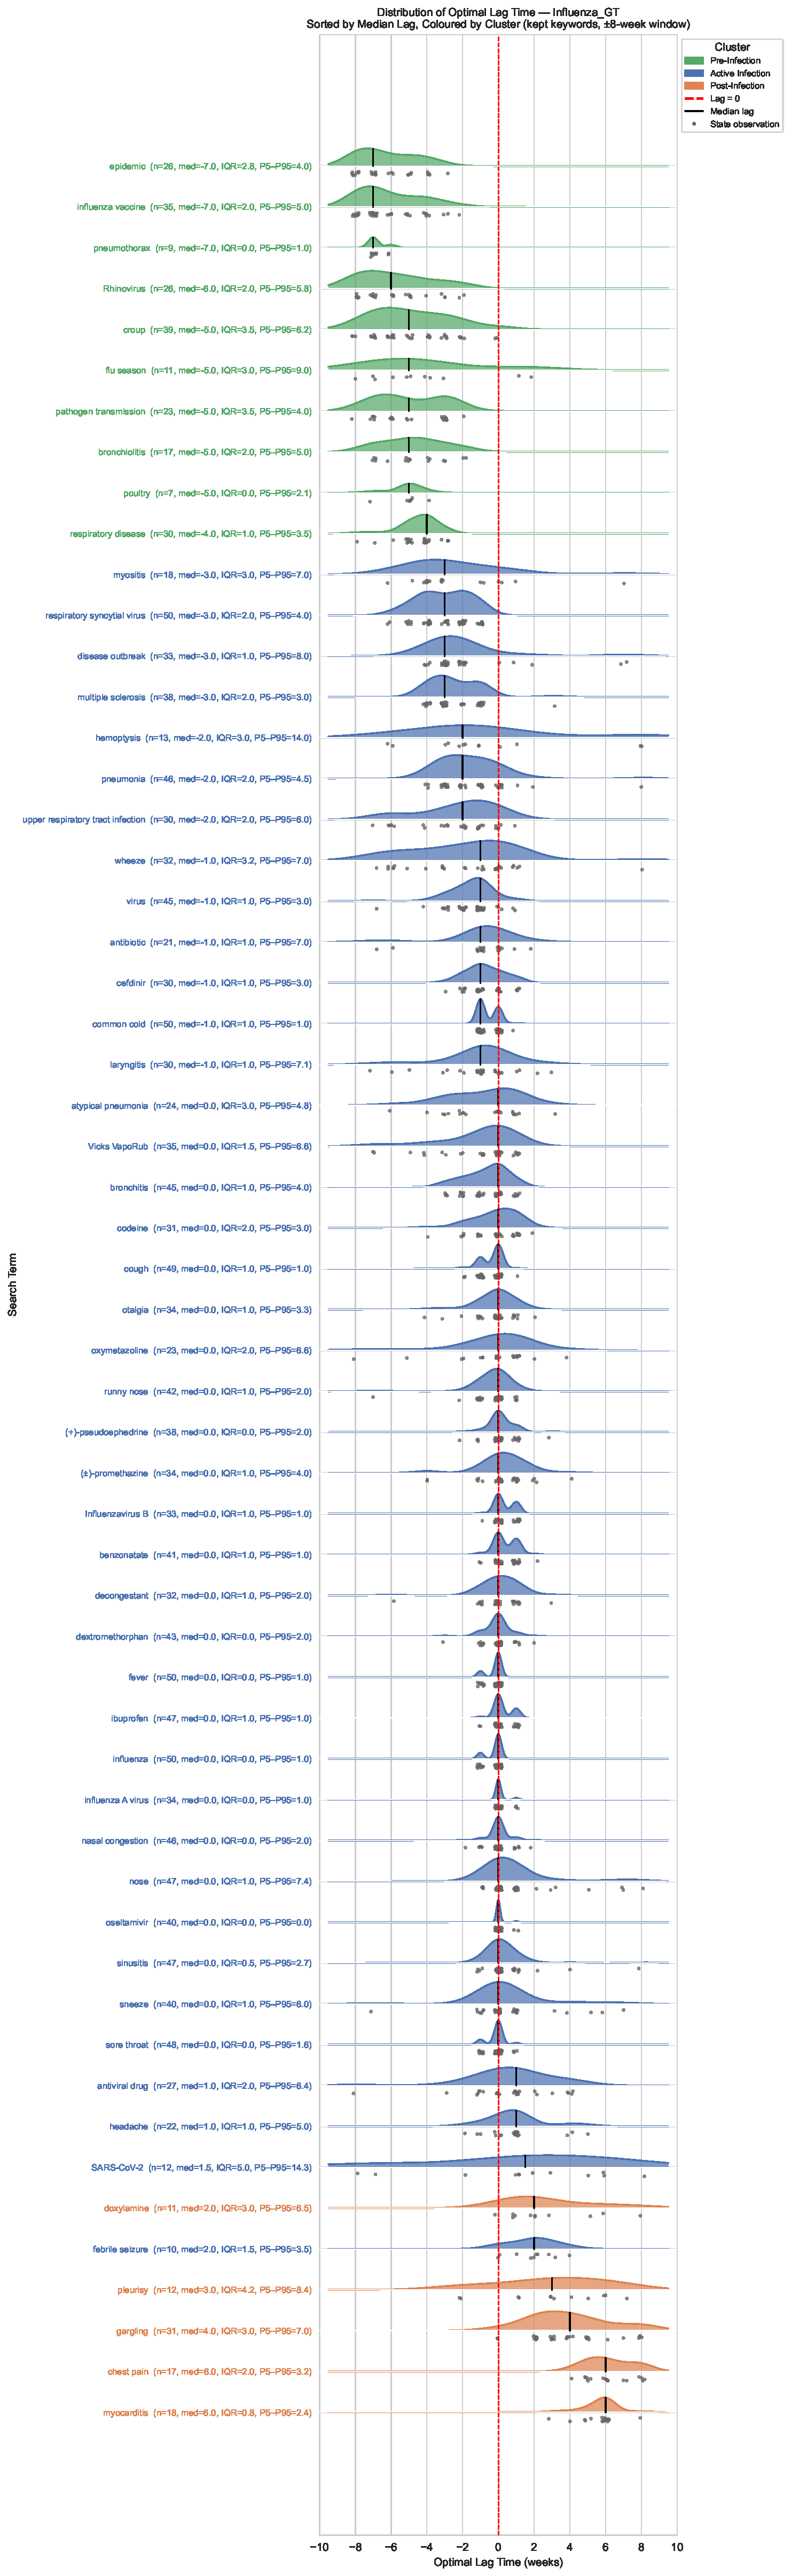
\includegraphics[height=0.66\textheight]{figs/ridgeline_flu_gt.pdf}
    \end{column}
    \begin{column}{0.46\textwidth}
      Related queries sort into three stages by their lag to ED visits:
      \begin{itemize}
        \item \textbf{Pre} (prevention): leads by \textbf{4--7 weeks},
        \item \textbf{Active} (symptoms, acute care): about \textbf{0},
        \item \textbf{Post} (complications): lags by \textbf{3--5 weeks}.
      \end{itemize}
      Holds across Google Trends \emph{and} clinician (UpToDate) searches, for both
      influenza and RSV, in over 90\% of states.
    \end{column}
  \end{columns}
\end{frame}

\begin{frame}{The three composites track the wave at different offsets}
  \begin{center}
    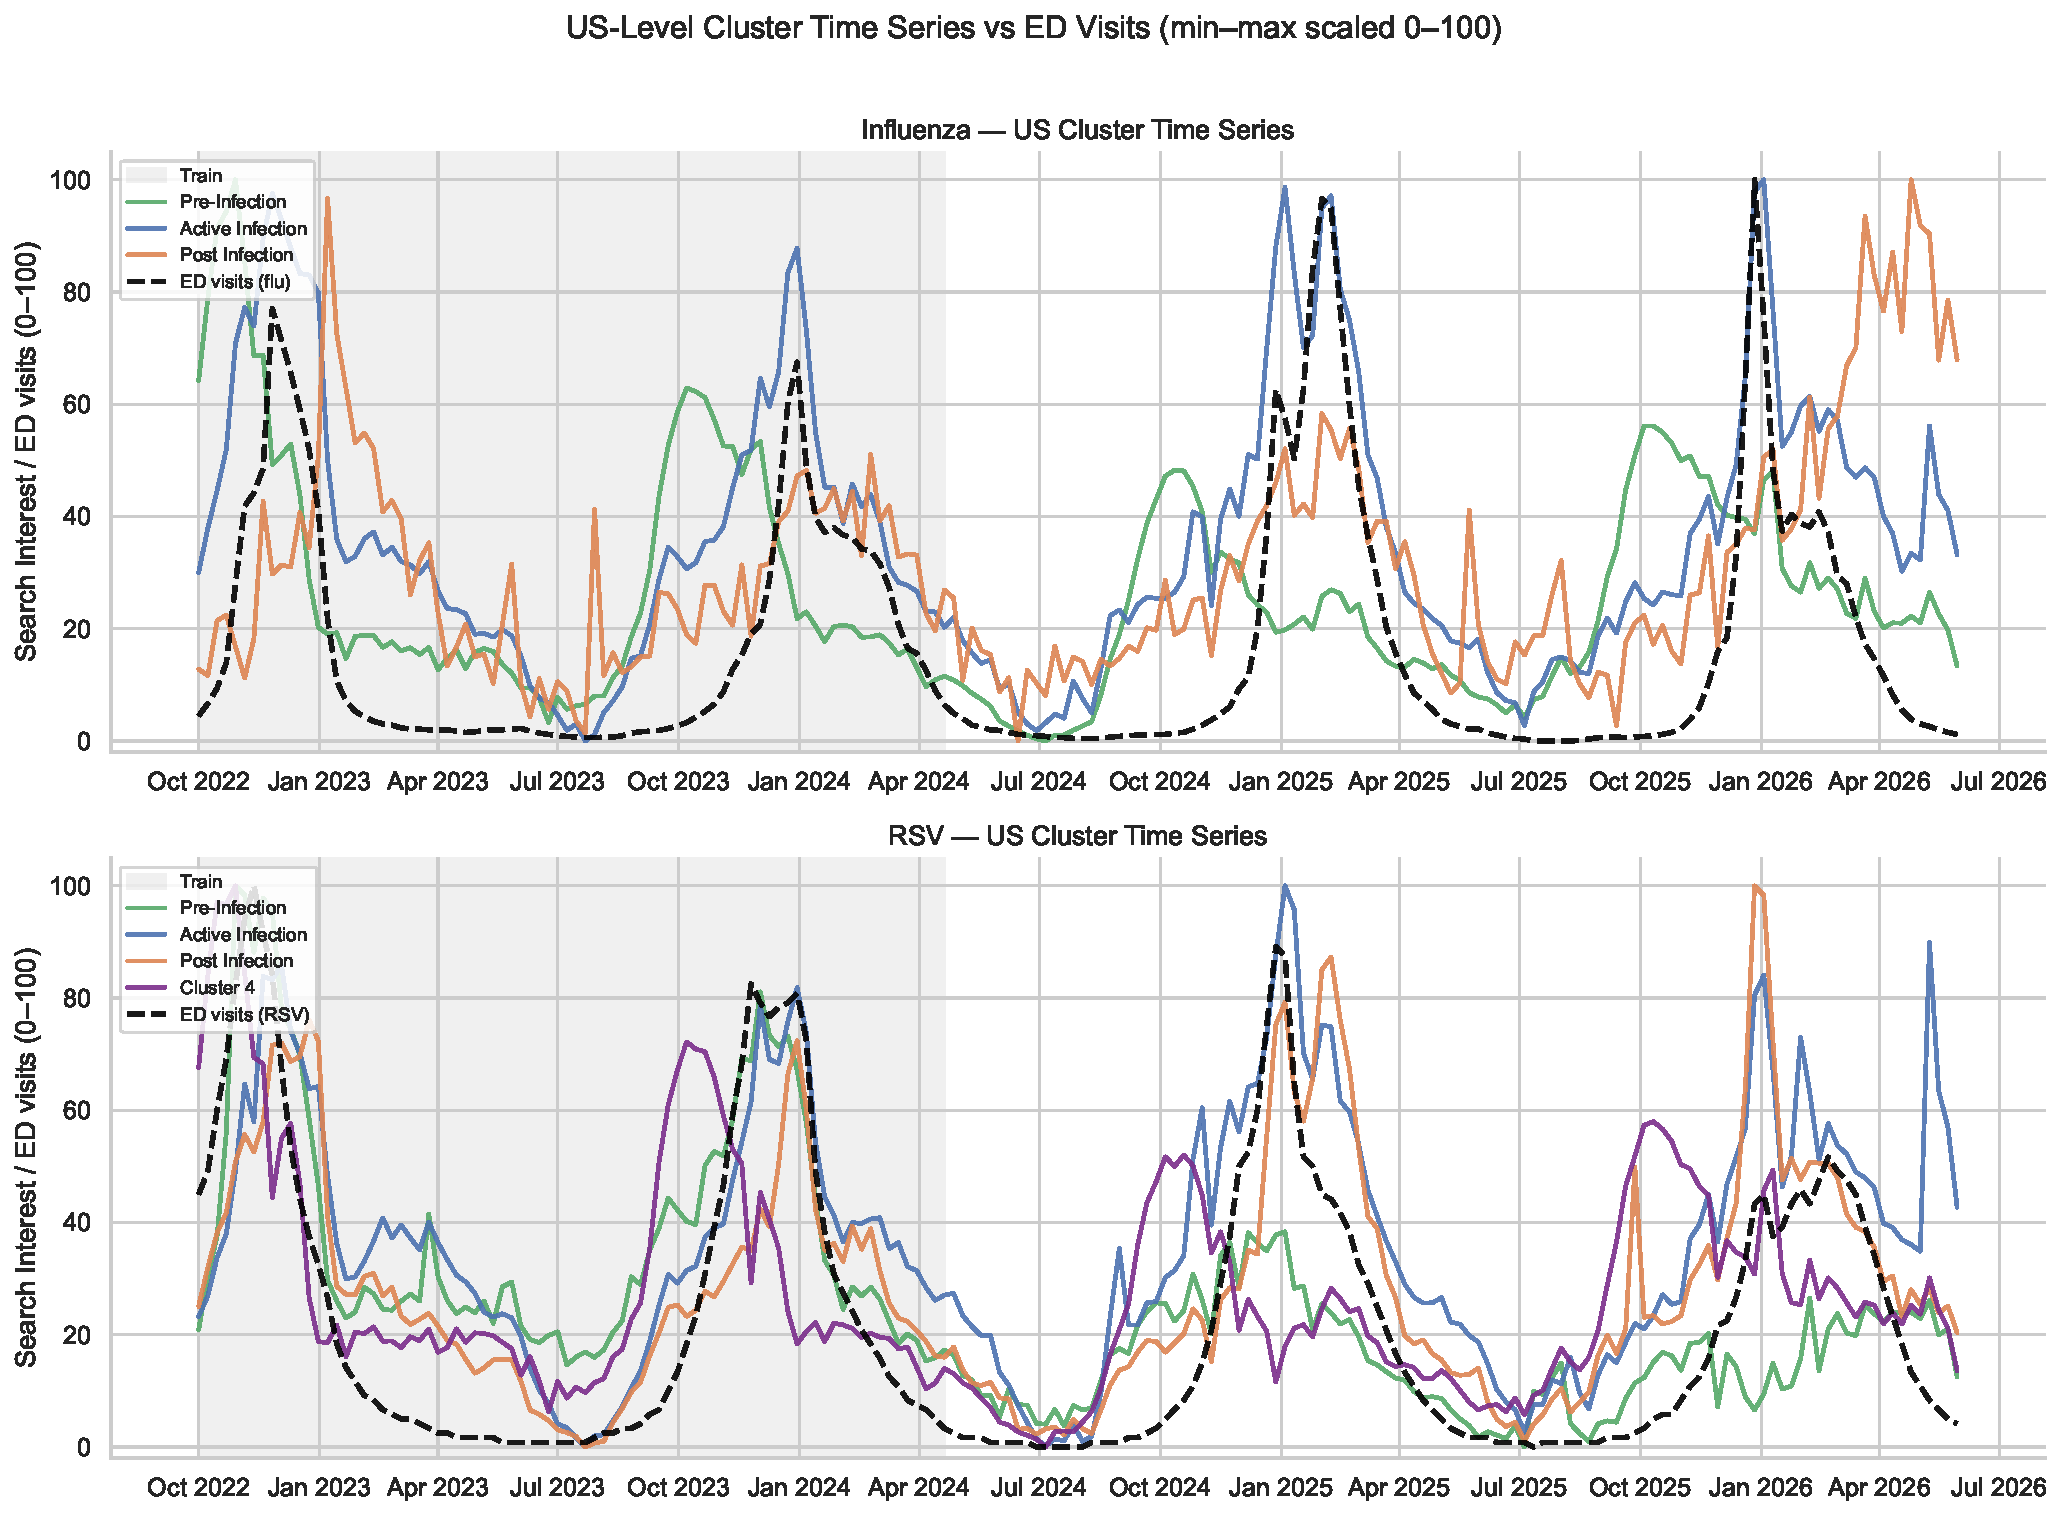
\includegraphics[height=0.72\textheight]{figs/composite_vs_ed.pdf}
  \end{center}
  \vspace{-0.2em}
  \begin{center}
    \itshape Pre leads, Active is on-peak, Post trails, all overlaid on ED visits.
  \end{center}
\end{frame}

\begin{frame}{Why the stage view matters}
  \begin{itemize}
    \item It is not just ``search predicts cases.'' The \emph{category} of search tells you
          \textbf{which stage} of the outbreak you are in.
    \item Different stages help at different \textbf{forecast horizons}: prevention terms
          for longer lead times, symptom terms for the near term.
    \item It replicates across a completely different data source (clinician searches), so
          it is a \textbf{real epidemiological structure}, not a Google Trends artifact.
  \end{itemize}
  \vspace{0.3em}
  \begin{alertblock}{Two honest caveats}
    Search reflects attention, not only infection (news moves it too), and relationships
    drift as a disease becomes familiar. Preprocess, validate out of sample, re-check each
    season.
  \end{alertblock}
\end{frame}

% ===============================================================
\section{Wrap-up}

\begin{frame}{Google Trends field guide (screenshot this)}
  \begin{itemize}
    \item Never trust a \textbf{single raw pull}: pull repeatedly and average.
    \item Prefer \textbf{topics} over raw strings.
    \item \textbf{Combine} related terms; drop columns that are mostly zeros.
    \item \textbf{Denoise} (smoothing) and \textbf{detrend} (remove pipeline drift).
    \item Expect quality to \textbf{drift over time}; re-validate old pipelines.
    \item Always judge on \textbf{out-of-sample} forecast error, not in-sample fit.
  \end{itemize}
  \vspace{0.3em}
  \begin{center}
    \itshape Raw Google Trends can hurt a model. Preprocessed, it is a genuine early signal.
  \end{center}
\end{frame}

\begin{frame}{Looking ahead}
  \begin{itemize}
    \item \textbf{Next (3:30):} use an agent to scrape more streams (Wikipedia, wastewater)
          the same careful way.
    \item \textbf{Day 2:} feed these \emph{preprocessed}, stage-grouped search signals into
          \textbf{ARGO}, alongside the disease's own history.
  \end{itemize}
  \vfill
  \begin{center}
    \itshape You now know both how to get a Google Trends signal and how to make it
    trustworthy. That is most of the battle.
  \end{center}
\end{frame}

\begin{frame}[standout]
  Questions?
\end{frame}

\end{document}
